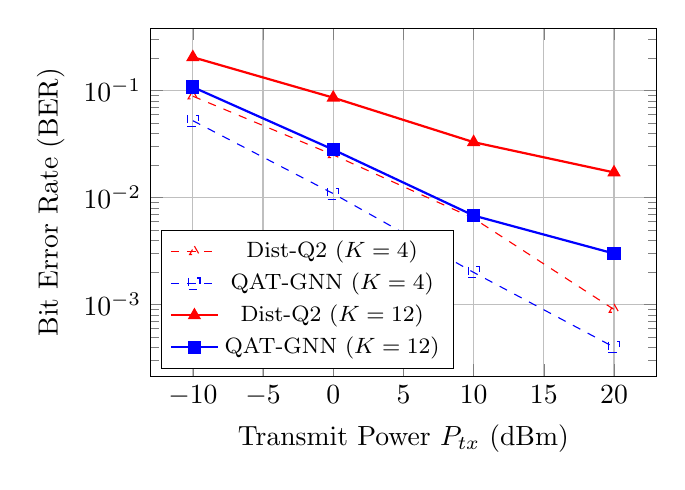
\begin{tikzpicture}
\begin{semilogyaxis}[
    xlabel={Transmit Power $P_{tx}$ (dBm)},
    ylabel={Bit Error Rate (BER)},
    grid=major,
    legend style={at={(0.02,0.02)}, anchor=south west, font=\footnotesize},
    width=8cm,
    height=6cm
]

% K=4 Dist-Q2
\addplot[color=red, mark=triangle, dashed] coordinates {
    (-10, 0.0888) (0, 0.0251) (10, 0.0064) (20, 0.0009)
};
\addlegendentry{Dist-Q2 ($K=4$)}

% K=4 QAT-GNN
\addplot[color=blue, mark=square, dashed] coordinates {
    (-10, 0.0524) (0, 0.0109) (10, 0.0020) (20, 0.0004)
};
\addlegendentry{QAT-GNN ($K=4$)}

% K=12 Dist-Q2
\addplot[color=red, mark=triangle*, thick] coordinates {
    (-10, 0.2054) (0, 0.0860) (10, 0.0330) (20, 0.0172)
};
\addlegendentry{Dist-Q2 ($K=12$)}

% K=12 QAT-GNN
\addplot[color=blue, mark=square*, thick] coordinates {
    (-10, 0.1080) (0, 0.0281) (10, 0.0068) (20, 0.0030)
};
\addlegendentry{QAT-GNN ($K=12$)}

\end{semilogyaxis}
\end{tikzpicture}